\documentclass{article}

% Language setting
% Replace `english' with e.g. `spanish' to change the document language
\usepackage[english]{babel}

% Set page size and margins
% Replace `letterpaper' with `a4paper' for UK/EU standard size
\usepackage[letterpaper,top=2cm,bottom=2cm,left=3cm,right=3cm,marginparwidth=1.75cm]{geometry}

% Useful packages
\usepackage{amsmath}
\usepackage{graphicx}
\usepackage[colorlinks=true, allcolors=blue]{hyperref}
\usepackage{amssymb}
\usepackage{hyperref}
\usepackage{nameref}
\usepackage{amsmath,amssymb}
\usepackage{amsfonts}
\usepackage{graphicx}
\usepackage{enumerate}
\usepackage{xcolor,colortbl}
\usepackage{times}
\usepackage{pgf}
\usepackage{amsfonts}
\usepackage{subcaption}
\usepackage{authblk}
\usepackage{floatflt}
\usepackage{graphicx}
\usepackage{array}
\usepackage{caption}
\usepackage{verbatim}
\usepackage{caption}
\DeclareMathOperator*{\argmax}{arg\,max}

\DeclareCaptionType{equ}[][]
%\captionsetup[equ]{labelformat=empty}

% Pseudo code %
\usepackage{amsmath}
\usepackage{algorithm}
\usepackage[noend]{algpseudocode}
\algdef{SE}{Begin}{End}{\textbf{begin}}{\textbf{end}}

\title{Current Progress, Problems and future Ideas regarding Ecoli-Tracking}
\author{Elias Pinter}
\begin{document}
\maketitle

\section{Detection}
The approach that i have been using for detection actually does not use machine learning at all as it mainly exploits the fact
that the background of a typical recording does not change. It is semi-automatic since it requires that the first frame of the video
is labeled by hand. The Ecoli are then removed from the first frame via inpainting and some image processing to get a clean picture
of the background. This image of the background can then be used to subtract from it from any frame in the video to obtain the Ecoli with some
more image processing. The two code snippets \textbf{Alogrithm 1} and  \textbf{Alogrithm 2} below describe the creation of the template and
the detection process in an abstract way in pseudo code notation.


% \begin{algorithm}[hbt!]
%     \caption{Creation of template}\label{alg:two}
%     \KwData{labels, gray\_image, first\_image} 
%     \For{label}{
%         $x, y, w, h \gets \mathit{label}$\\
%         Store label for tracking\\
%         \Comment{Ecoli is obtained by threshholding within the box}
%         $\mathit{temp\_mask} \gets \mathit{gray\_image}[y:y + h, x:x + w] < \mathit{threshhold}$\\
%         $\textit{mask}[y:y + h, x:x + w] \gets \mathit{temp\_mask}$
%     }
%     $\textit{template} \gets \mathit{inpaint(first\_image, mask, radius)}$\\
%     \For{label}{
%         $x, y, w, h \gets \mathit{label}$\\
%         $\mathit{roi} \gets \mathit{template[y:y+h+increase, x:x+w+increase]}$\\
%         \Comment{Blurring is performed around the inpainted region to smoothen the image}
%         $\mathit{GaussianBlur(roi)}$
%     }
% \end{algorithm}

\begin{algorithm}
    \caption{Creates a template by ipainting the user labeled Ecoli
    and blurring the neighbouring regions}
    \label{alg:template}
    \renewcommand{\thealgorithm}{}
    \floatname{algorithm}{}
    \begin{algorithmic}[1]
        \For{label}
            \State $x, y, w, h \gets \mathit{label}$
            \State Store label for tracking
            \State $\mathit{temp\_mask} \gets \mathit{gray\_image}[y:y + h, x:x + w] < \mathit{threshhold}$ \Comment{Obtain Ecoli via Thresholding}
            \State $\textit{mask}[y:y + h, x:x + w] \gets \mathit{temp\_mask}$
        \EndFor
        \State $\textit{template} \gets \mathit{inpaint(first\_image, mask, radius)}$
        \For{label}
            \State $x, y, w, h \gets \mathit{label}$
            \State $\mathit{roi} \gets \mathit{template[y:y+h+increase, x:x+w+increase]}$\\
        \Comment{Blurring is performed around the inpainted region to smoothen the image}
            \State $\mathit{GaussianBlur(roi)}$
        \EndFor
        \State \Return template
\end{algorithmic}\end{algorithm}

\begin{figure}
    \centering
    \begin{subfigure}[b]{.45\linewidth}
    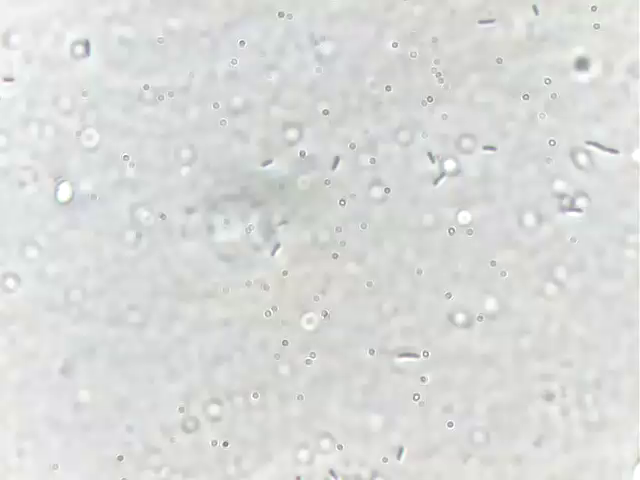
\includegraphics[width=\linewidth]{image000000.png}
    \caption{Original Image}\label{fig:original}
    \end{subfigure}
    \begin{subfigure}[b]{.45\linewidth}
    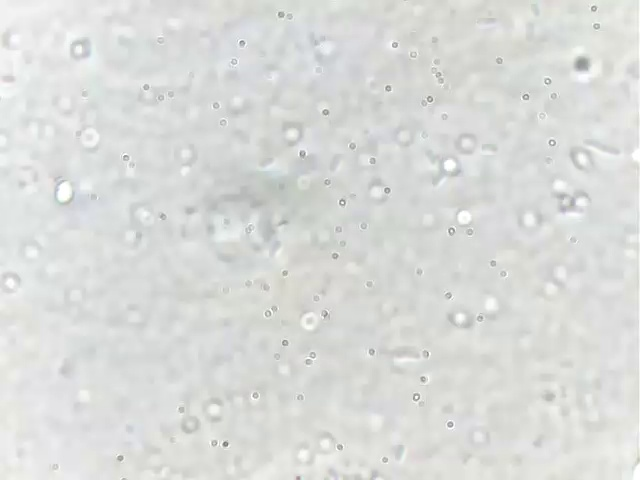
\includegraphics[width=\linewidth]{template.jpg}
    \caption{Template}\label{fig:template}
    \end{subfigure}
    \caption{Template}
\end{figure}

\begin{algorithm}
    \caption{Detects Ecoli in a frame of the video using the template}
    \label{alg:detection}
    \renewcommand{\thealgorithm}{}
    \floatname{algorithm}{}
    \begin{algorithmic}[1]
        \State $\mathit{boxes} \gets \mathit{[\hspace{6px}]}$
        \State $\mathit{subtraction} \gets \mathit{subtract(template, image)}$
        \State $\mathit{subtraction} \gets \mathit{grayImage(subtraction)}$
        \State $\mathit{ecoli\_noisy} \gets \mathit{thresholding(subtraction, threshold)}$
        \State $\textit{ecoli} \gets \mathit{medianBlur(ecoli\_noisy, kernel\_size)}$
        \State $\textit{contours} \gets \mathit{findContours(ecoli)}$
        \For{contour}
            \State $x, y, w, h \gets \mathit{boundingRect(contour)}$
            \If{$w \leq \mathit{width\_cutoff } \lor h \leq \mathit{height\_cutoff}$}{
                continue    
            } \Comment{Skip boxes that are too small} 
            \EndIf
            \State $x \gets x-1$ \Comment{Make up for subtraction}
            \State $y \gets y-1$
            \State $w \gets w+2$
            \State $h \gets h+2$
            \State $\mathit{boxes.append((x, y, w, h))}$
        \EndFor
        \State \Return boxes
\end{algorithmic}\end{algorithm}

\renewcommand\thesubfigure{\roman{subfigure}}
\begin{figure}
    \centering
    \begin{subfigure}[b]{.45\linewidth}
    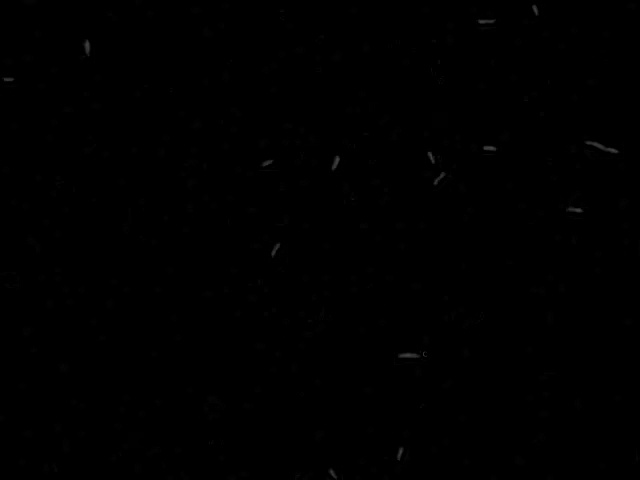
\includegraphics[width=\linewidth]{subtraction.jpg}
    \caption{Subtraction}\label{fig:subtraction}
    \end{subfigure}
    \begin{subfigure}[b]{.45\linewidth}
    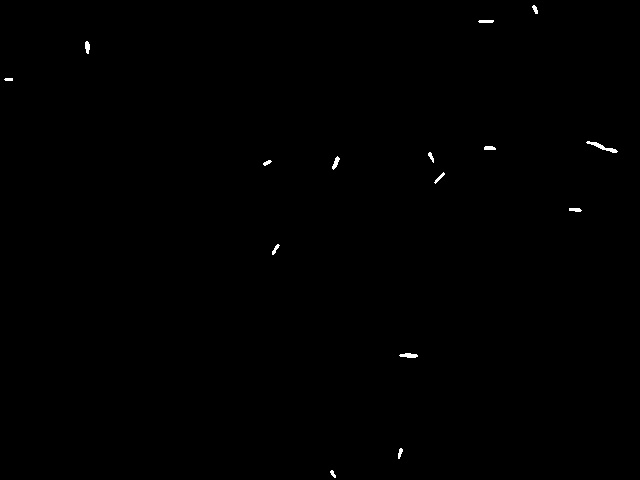
\includegraphics[width=\linewidth]{threshold.jpg}
    \caption{Threshholded Image}\label{fig:threshold}
    \end{subfigure}

    \begin{subfigure}[b]{.45\linewidth}
    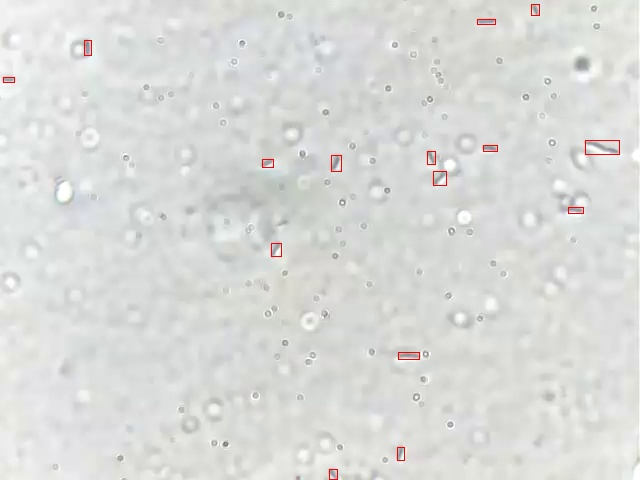
\includegraphics[width=\linewidth]{boxes.jpg}
    \caption{Detections}\label{fig:detecions}
    \end{subfigure}
    \caption{Detection Process}
\end{figure}

\section{Tracking}
The current tracking approach is IoU based and makes use of domain knowledge
about the ecperimental setup. The algorithm is based on the following four assumptions:
\begin{itemize}
    \item Ecoli stay in there local environment since there are no cuts
    in the video
    \item Ecoli can only appear on the edge of the window
    \item Ecoli can only disappear on the edge of the window
    \item Ecoli can only seperate and never merge
\end{itemize}
Since it is not guranteed that our detection obeys these assumptions we need to know
when certain events happen and handle them explicitely in our tracking algorithm.
\subsection[short]{Definitions}
For describing the tracking algorithm we first need to through a couple
of definitions. We will first start with bounding boxes. There will be two different ways
of referring to bounding boxes dpepending on whether the Id of the bounding box
is known. Id the id is not known yet we will refer to the boxes via indices.
\begin{equ}[!ht]
    \begin{equation*}
      b_{t}^i
    \end{equation*}
  \caption{Box with Id $i$ at the frame $t$}
\end{equ}
\begin{equ}[!ht]
    \begin{equation*}
      b_{t, k}
    \end{equation*}
  \caption{Box with yet unknown Id with index $k$ at the frame $t$}
\end{equ}\\
For the general tracking and to recognize if a certain event happened we will use two metrics, which we will also define, namely IoU(Intersection over Union)
and IoA(Intersection over Area). Let $A(x)$ denote a function that returns the Area of a rectangle then we define for two boxes $x$ and $y$
\begin{align*}
    IoU(x,y) &:= \frac{A(x \cap y)}{A(x \cup y)}\\
    IoA(x,y) &:= \frac{A(x \cap y)}{A(y)} 
\end{align*}
\subsection[short]{General Mapping and Important Events}
First of all we will define the general mapping strategy to map boxes with Ids from a frame $t$ to the boxes without Ids in frame $t+1$. We will map a box $b_{t}^i$
to the box $b_{t+1, k}$ if $b_{t+1, k}$ maximizes the IoU score for $b_{t}^i$ and is above a certain threshold. Let the general mapping be called $f$ then we can
define it in the following way:
\begin{align}
    f \left(b_{t}^i \right) = b_{t+1, k'} \text{ where } k' := \argmax_k \; IoU \left(b_{t}^i, b_{t+1, k}\right) \text{ if } IoU \left(b_{t}^i, b_{t+1, k'}\right) > threshold  
\end{align}   
When tracking there are a couple of important events that we need to recognize. Those are
\begin{enumerate}[i.]
    \item sudden appearance of cell
    \item sudden disappearance of cell
    \item merging of boxes
    \item cell duplication 
\end{enumerate}
the following statments describe how we will detect that one of those events happened. For i. we will say that a box at time $t+1$ appeared if there is no box at time
$t$ that maps onto it. So we say that box $b_{t+1, k}$ just appeared if fulfills the follwoing statement.
\begin{align}
    \nexists i \; f\left(b_{t}^i\right) = b_{t+1, k}
\end{align}
Similarly for ii. we say that a box $b_{t}^i$ at frame $t$ disappeared if there is no box in frame $t+1$ it maps onto. This means $b_{t}^i$ disappeared if ot fulfills
the statement
\begin{align}
    \nexists k \; f\left(b_{t}^i\right) = b_{t+1, k}
\end{align}
For event iii. we say that two boxes merged into a box at frame $t+1$ if they both map onto to the same box under $f$. This means that boxes $b_{t}^i$ and $b_{t}^j$
merged into a box $b_{t+1, k}$ if the follwoing statement holds
\begin{align}
    f\left(b_{t}^i\right) = f\left(b_{t}^j\right) = b_{t+1, k} \text{ with } j \neq k
\end{align}
Note that this statement can easily be expanded to more then two boxes.\\
For cell duplication we say that it took place if there are two boxes $b_{t+1, j}$ and $b_{t+1, k}$ whose IoA score relative to a box $b_{t}^i$ is above a certain threshhold.
\begin{align}
    \exists j, k \; IoA(b_{t}^i, b_{t+1, j}) > threshold \land IoA(b_{t}^i, b_{t+1, k}) > threshold \text{ with } j \neq k
\end{align}
Now we have the fundamental building blocks for the tracking algorithm that is decribed below in \textbf{Algorithm 3}. For finding boxes that disappeared or were
part of a merge we will perform a sliding window search with it's old image in the neighbourhood of its old box in the new image. It is also imortant to mention
that we will only search for disappeared boxes if they were not close to the border and that we will ignore boxes that were not close to the border when they appeared. 
For the first frame of the video every box from the user labeling gets assigned an Id.\medskip\\
\newpage
\noindent For the following Algorithm let $\max(I)$ denote denote a function that returns the highest previously assigned Id. $B_t$ will describe the set of boxes at time $t$.  
\begin{algorithm}
    \caption{Tracks Ecoli between frames $t$ and $t+1$}
    \label{alg:tracking}
    \renewcommand{\thealgorithm}{}
    \floatname{algorithm}{}
    \begin{algorithmic}[1]
        \State $\mathit{detections} \gets \mathit{detect(image_{t+1})}$
        \State $\mathit{mapping} \gets \mathit{\{\;\}}$
        \State $\mathit{duplicated} \gets \mathit{\mathit{\{\;\}}}$
        \State $\mathit{merged} \gets \mathit{\mathit{\{\;\}}}$
        \For{$b_{t}^i \in B_t$}
            \For{$b_{t+1, k} \in detections$}{}
                \Comment{Calculate all pairwise metrics}
                \State $IoU(b_{t}^i, b_{t+1, k})$
                \State $IoA(b_{t}^i, b_{t+1, k})$
            \EndFor
            \Comment{Check if box duplicated}
            \If{(5) for $b^i_t$}
                \State $\mathit{new\_id} \gets \max (I_t) + 1$
                \State $B_{t+1} \cup b_{t+1}^{new\_id}$    
                \State $\mathit{new\_id} \gets \max (I_t) + 1$
                \State $B_{t+1} \cup b_{t+1}^{new\_id}$
                \State $\mathit{duplicated} \gets \mathit{duplicated} \cup i$    
            \EndIf
        \EndFor
        \If{$\displaystyle \max_{k} IoU\left(b_{t}^i, b_{t+1, k}\right) < threshold$}
            continue 
        \EndIf
        \For{$b_{t}^i$ that statisfy (4)} \Comment{Find merged boxes with sliding window search}
            \State $new\_box \gets \mathit{sliding\_window\_search\left(b_{t}^i\right)}$
            \State $B_{t+1} \gets B_{t+1} \cup \mathit{new\_box}$
            \State $\mathit{merged} \gets \mathit{merged} \cup i$ 
        \EndFor
        \For{$b_{t+1, k}$ that statisfy (2)} \Comment{Check if boxes appeared close to the border}
            \If{$\mathit{distance\_to\_border(b_{t+1, k})} < threshold$}
                \State $\mathit{new\_id} \gets \max (I) + 1$
                \State $b_{t+1}^{new\_id} \gets b_{t+1, k}$
                \State $B_{t+1} \gets B_{t+1} \cup \mathit{b_{t+1}^{new\_id}}$ 
            \EndIf
        \EndFor
        \For{$b_{t}^i$ that statisfy (3)} \Comment{Check if boxes disappeared far from the border}
            \If{$\mathit{distance\_to\_border(b_{t}^i)} \geq threshold$}
                \State $new\_box \gets \mathit{sliding\_window\_search\left(b_{t}^i\right)}$
                \State $B_{t+1} \gets B_{t+1} \cup \mathit{new\_box}$ 
            \EndIf
        \EndFor
        \Comment{All old boxes that were not merged or duplicated get mapped according to (1)}
        \For{$b_{t}^i$ where $i \not \in (\mathit{duplicated} \cup \mathit{merged}) $} 
            \State $B_{t+1} \gets B_{t+1} \cup f(b_{t}^i)$ 
        \EndFor
\end{algorithmic}\end{algorithm}\\
This algorithm can be performed for successive frames until the last frame of the vidoe has its mapping.
In the source code which can be found \href{https://github.com/BioDisCo/ecolitracking}{here}. There is also a
modified version of the BioPython library being used to create a population forest of the tracked Ecoli. If you have
any questions regarding the source code just contact me on Discord: elson1608. 

\section{Experimental Setup}
\subsection{Problems}
The problems we faced regarding the experimental setup are the follwoing
\begin{itemize}
    \item Channel dries out
    \item Focus Drift
\end{itemize} 
For the first one we first tried to stick two cones filled with LB in the two holes of the microfluidic channel.
This did not really work since LB seems to be too thick. However when we tried the same with water it worked quite well.
The only interesting thing about the water solution was that many Ecoli got "gravitated" towards the two holes.
\medskip\\
For the Focus drift we haven't really found a solution yet there are two causes that we suspect to be responsible
for the loss of focus
\begin{itemize}
    \item Temperature Fluctuations
    \item Stage Drift 
\end{itemize}
Regarding the temperature fluctuations we measured the room temperature over the weekend and it seems like there is a
difference of one degree Celsius between day and night as can be seen in \textbf{Figure 3}.
\medskip\\
\begin{figure}[!h]
    \centering
    \begin{subfigure}[b]{.35\linewidth}
    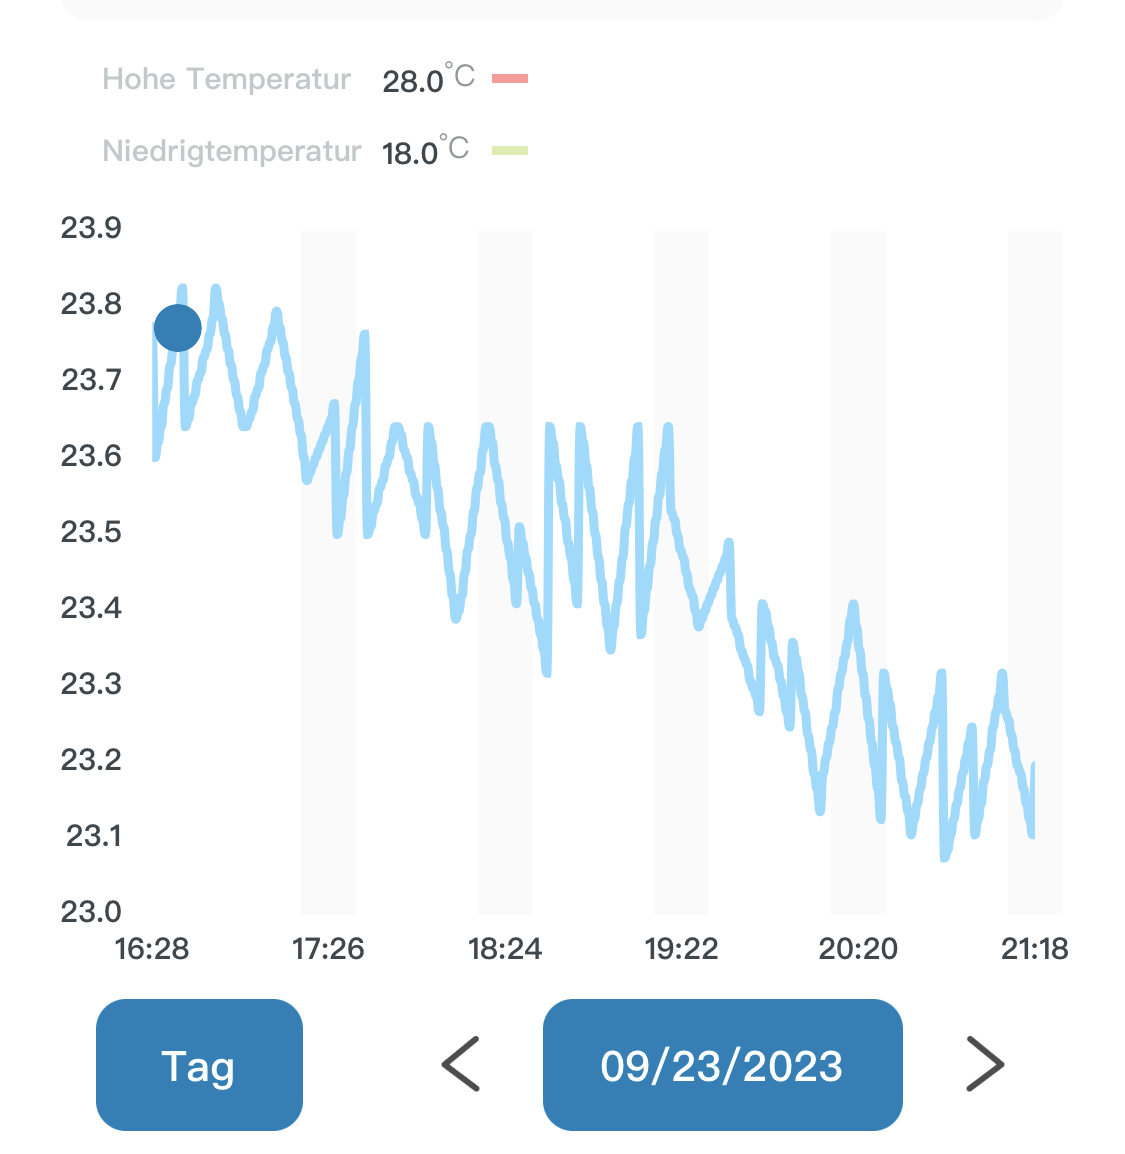
\includegraphics[width=\linewidth]{9_23.png}
    \end{subfigure}
    \begin{subfigure}[b]{.35\linewidth}
    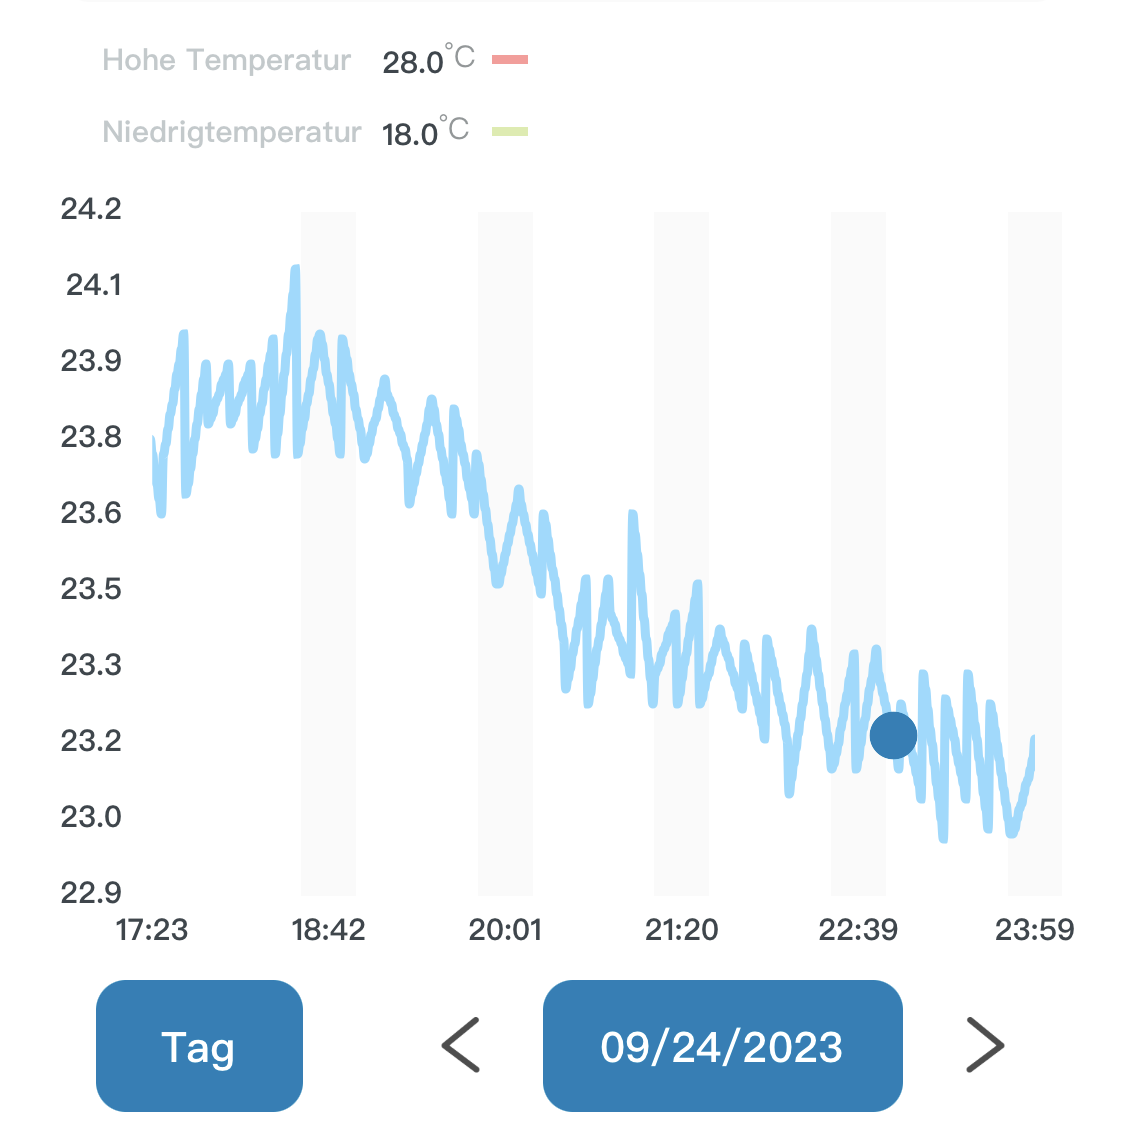
\includegraphics[width=\linewidth]{9_24.png}
    \end{subfigure}
    \caption{Temperature Fluctuations}
\end{figure}\\

Something else that we are trying to find out is during which stage in their lifecycle the Ecoli have the darkest color,
since a high contrast is very beneficial for detection. 
\section{Possible Ideas for future Work}
Regarding future work the most important thing will probably be to increase the quality of the videos and tackle the problems
mentioned in \textbf{3}. Also one could try to find an alternative to the sliding window search that works better. Using the Watershed
Alogrithm in very large boundg boxes during the detection stage could help at preventing merges and spotting duplication earlier.
Also it could be interesting to look at mixed scenarios with Algae and Ecoli together.
\end{document}